%\section{BEE 1195 -- Árvore Binária de Busca}

\begin{frame}[fragile]{Problema}

Em computação, a árvores binária de busca ou árvore binária de pesquisa é uma estrutura baseada em nós (nodos), onde todos os nós da subárvore esquerda possuem um valor numérico inferior ao nó raiz e todos os nós da subárvore direita possuem um valor superior ao nó raiz (e assim sucessivamente). O objetivo desta árvore é estruturar os dados de forma flexível, permitindo a busca binária de um elemento qualquer da árvore.

A grande vantagem das árvores de busca binária sobre estruturas de dados convencionais é que os algoritmos de ordenação (percurso infixo) e pesquisa que as utilizam são muito eficientes.

Para este problema, você receberá vários conjuntos de números e a partir de cada um dos conjuntos, deverá construir uma árvore binária de busca. Por exemplo, a sequência de valores: 8 3 10 14 6 4 13 7 1 resulta na seguinte árvore binária de busca:

\end{frame}

\begin{frame}[fragile]{Problema}

    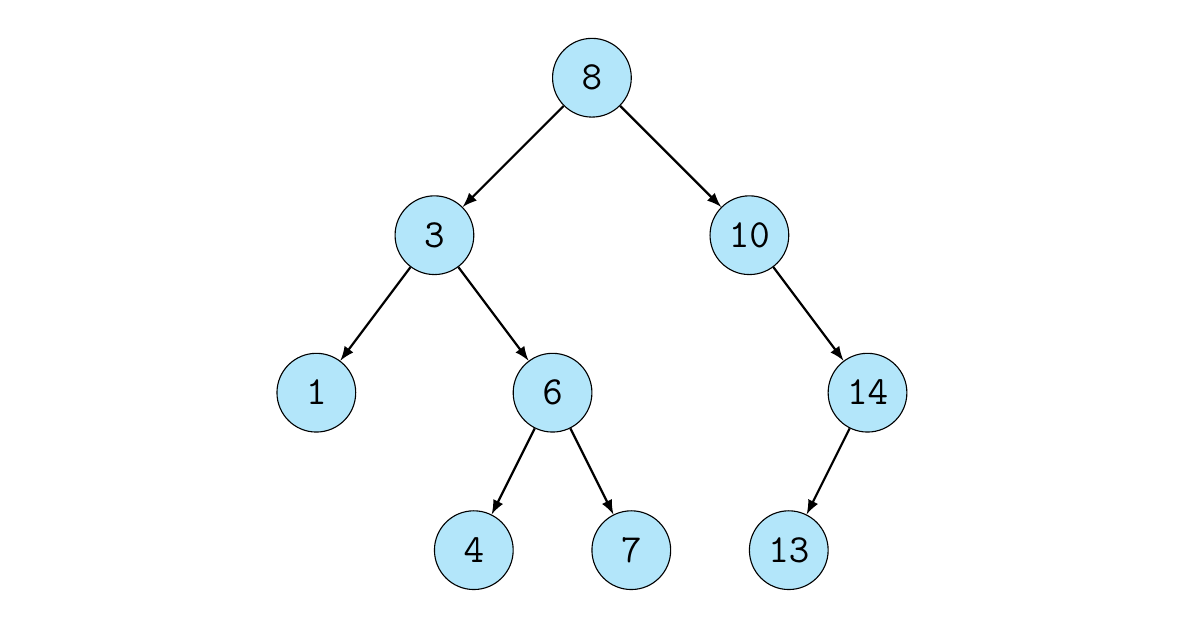
\begin{tikzpicture}
            \node[opacity=0] at (0, 7) { . };
            \node[opacity=0] at (14, 0) { . };

            \node[circle,draw,fill=cyan!30,minimum size=1cm] (A) at (7, 6.5) { \Large \tt 8 };
            \node[circle,draw,fill=cyan!30,minimum size=1cm] (B) at (5, 4.5) { \Large \tt 3 };
            \node[circle,draw,fill=cyan!30,minimum size=1cm] (C) at (9, 4.5) { \Large \tt 10 };
            \node[circle,draw,fill=cyan!30,minimum size=1cm] (D) at (3.5, 2.5) { \Large \tt 1 };
            \node[circle,draw,fill=cyan!30,minimum size=1cm] (E) at (6.5, 2.5) { \Large \tt 6 };
            \node[circle,draw,fill=cyan!30,minimum size=1cm] (F) at (10.5, 2.5) { \Large \tt 14 };
            \node[circle,draw,fill=cyan!30,minimum size=1cm] (G) at (5.5, 0.5) { \Large \tt 4 };
            \node[circle,draw,fill=cyan!30,minimum size=1cm] (H) at (7.5, 0.5) { \Large \tt 7 };
            \node[circle,draw,fill=cyan!30,minimum size=1cm] (I) at (9.5, 0.5) { \Large \tt 13 };

            \draw[-latex,thick] (A) to (B);
            \draw[-latex,thick] (A) to (C);
            \draw[-latex,thick] (B) to (D);
            \draw[-latex,thick] (B) to (E);
            \draw[-latex,thick] (C) to (F);
            \draw[-latex,thick] (E) to (G);
            \draw[-latex,thick] (E) to (H);
            \draw[-latex,thick] (F) to (I);
    \end{tikzpicture}

\end{frame}

\begin{frame}[fragile]{Entrada e saída}

\textbf{Entrada}

A entrada contém vários casos de teste. A primeira linha da entrada contém um inteiro $C$ $(C \leq 1000)$, indicando o número de casos de teste que virão a seguir. Cada caso de teste é composto por 2 linhas. A primeira linha contém um inteiro $N$ $(1 \leq N \leq 500)$ que indica a quantidade de números que deve compor cada árvore e a segunda linha contém $N$ inteiros distintos e não negativos, separados por um espaço em branco.

\textbf{Saída}

Cada linha de entrada produz 3 linhas de saída. Após construir a árvore binária de busca com os elementos de entrada, você deverá imprimir a mensagem "Case $n$:", onde $n$ indica o número do caso de teste e fazer os três percursos da árvore: prefixo, infixo e posfixo, apresentando cada um deles em uma linha com uma mensagem correspondente conforme o exemplo abaixo, separando cada um dos elementos por um espaço em branco. 

Obs: Não deve haver espaço em branco após o último item de cada linha e há uma linha em branco após cada caso de teste, inclusive após o último.

\end{frame}

\begin{frame}[fragile]{Exemplo de entradas e saídas}

\begin{minipage}[t]{0.5\textwidth}
\textbf{Exemplo de Entrada}
\begin{verbatim}
2
3
5 2 7
9
8 3 10 14 6 4 13 7 1
\end{verbatim}
\end{minipage}
\begin{minipage}[t]{0.45\textwidth}
\textbf{Exemplo de Saída}
\begin{verbatim}
Case 1:
Pre.: 5 2 7
In..: 2 5 7
Post: 2 7 5

Case 2:
Pre.: 8 3 1 6 4 7 10 14 13
In..: 1 3 4 6 7 8 10 13 14
Post: 1 4 7 6 3 13 14 10 8
\end{verbatim}
\end{minipage}
\end{frame}

\begin{frame}[fragile]{Solução com complexidade $O(N^2)$}

    \begin{itemize}
        \item A solução do problema tem início com a codificação de uma árvore binária de
            busca

        \item Além do construtor, é preciso implementar a rotina de inserção (a qual tem
            complexidade $O(S)$ no pior caso, onde $S$ é o tamanho da árvore)

        \item Além disso, é preciso implementar as três travessias por profundidade notáveis
            (cuja complexidade de cada travessia também é $O(S)$)

        \item Por fim, para cada caso de teste, basta instanciar uma árvore, inserir os elementos
            indicados e produzir a saída usando as travessias indicadas
   \end{itemize}

\end{frame}

\begin{frame}[fragile]{Solução AC com complexidade $O(N^2)$}
    \inputsnippet{cpp}{1}{20}{codes/BEE1195.cpp}
\end{frame}

\begin{frame}[fragile]{Solução AC com complexidade $O(N^2)$}
    \inputsnippet{cpp}{22}{40}{codes/BEE1195.cpp}
\end{frame}

\begin{frame}[fragile]{Solução AC com complexidade $O(N^2)$}
    \inputsnippet{cpp}{42}{58}{codes/BEE1195.cpp}
\end{frame}

\begin{frame}[fragile]{Solução AC com complexidade $O(N^2)$}
    \inputsnippet{cpp}{60}{79}{codes/BEE1195.cpp}
\end{frame}

\begin{frame}[fragile]{Solução AC com complexidade $O(N^2)$}
    \inputsnippet{cpp}{81}{102}{codes/BEE1195.cpp}
\end{frame}
